% Options for packages loaded elsewhere
\PassOptionsToPackage{unicode}{hyperref}
\PassOptionsToPackage{hyphens}{url}
\PassOptionsToPackage{dvipsnames,svgnames,x11names}{xcolor}
%
\documentclass[
  letterpaper,
  DIV=11,
  numbers=noendperiod]{scrartcl}

\usepackage{amsmath,amssymb}
\usepackage{iftex}
\ifPDFTeX
  \usepackage[T1]{fontenc}
  \usepackage[utf8]{inputenc}
  \usepackage{textcomp} % provide euro and other symbols
\else % if luatex or xetex
  \usepackage{unicode-math}
  \defaultfontfeatures{Scale=MatchLowercase}
  \defaultfontfeatures[\rmfamily]{Ligatures=TeX,Scale=1}
\fi
\usepackage{lmodern}
\ifPDFTeX\else  
    % xetex/luatex font selection
\fi
% Use upquote if available, for straight quotes in verbatim environments
\IfFileExists{upquote.sty}{\usepackage{upquote}}{}
\IfFileExists{microtype.sty}{% use microtype if available
  \usepackage[]{microtype}
  \UseMicrotypeSet[protrusion]{basicmath} % disable protrusion for tt fonts
}{}
\makeatletter
\@ifundefined{KOMAClassName}{% if non-KOMA class
  \IfFileExists{parskip.sty}{%
    \usepackage{parskip}
  }{% else
    \setlength{\parindent}{0pt}
    \setlength{\parskip}{6pt plus 2pt minus 1pt}}
}{% if KOMA class
  \KOMAoptions{parskip=half}}
\makeatother
\usepackage{xcolor}
\setlength{\emergencystretch}{3em} % prevent overfull lines
\setcounter{secnumdepth}{-\maxdimen} % remove section numbering
% Make \paragraph and \subparagraph free-standing
\makeatletter
\ifx\paragraph\undefined\else
  \let\oldparagraph\paragraph
  \renewcommand{\paragraph}{
    \@ifstar
      \xxxParagraphStar
      \xxxParagraphNoStar
  }
  \newcommand{\xxxParagraphStar}[1]{\oldparagraph*{#1}\mbox{}}
  \newcommand{\xxxParagraphNoStar}[1]{\oldparagraph{#1}\mbox{}}
\fi
\ifx\subparagraph\undefined\else
  \let\oldsubparagraph\subparagraph
  \renewcommand{\subparagraph}{
    \@ifstar
      \xxxSubParagraphStar
      \xxxSubParagraphNoStar
  }
  \newcommand{\xxxSubParagraphStar}[1]{\oldsubparagraph*{#1}\mbox{}}
  \newcommand{\xxxSubParagraphNoStar}[1]{\oldsubparagraph{#1}\mbox{}}
\fi
\makeatother

\usepackage{color}
\usepackage{fancyvrb}
\newcommand{\VerbBar}{|}
\newcommand{\VERB}{\Verb[commandchars=\\\{\}]}
\DefineVerbatimEnvironment{Highlighting}{Verbatim}{commandchars=\\\{\}}
% Add ',fontsize=\small' for more characters per line
\usepackage{framed}
\definecolor{shadecolor}{RGB}{241,243,245}
\newenvironment{Shaded}{\begin{snugshade}}{\end{snugshade}}
\newcommand{\AlertTok}[1]{\textcolor[rgb]{0.68,0.00,0.00}{#1}}
\newcommand{\AnnotationTok}[1]{\textcolor[rgb]{0.37,0.37,0.37}{#1}}
\newcommand{\AttributeTok}[1]{\textcolor[rgb]{0.40,0.45,0.13}{#1}}
\newcommand{\BaseNTok}[1]{\textcolor[rgb]{0.68,0.00,0.00}{#1}}
\newcommand{\BuiltInTok}[1]{\textcolor[rgb]{0.00,0.23,0.31}{#1}}
\newcommand{\CharTok}[1]{\textcolor[rgb]{0.13,0.47,0.30}{#1}}
\newcommand{\CommentTok}[1]{\textcolor[rgb]{0.37,0.37,0.37}{#1}}
\newcommand{\CommentVarTok}[1]{\textcolor[rgb]{0.37,0.37,0.37}{\textit{#1}}}
\newcommand{\ConstantTok}[1]{\textcolor[rgb]{0.56,0.35,0.01}{#1}}
\newcommand{\ControlFlowTok}[1]{\textcolor[rgb]{0.00,0.23,0.31}{\textbf{#1}}}
\newcommand{\DataTypeTok}[1]{\textcolor[rgb]{0.68,0.00,0.00}{#1}}
\newcommand{\DecValTok}[1]{\textcolor[rgb]{0.68,0.00,0.00}{#1}}
\newcommand{\DocumentationTok}[1]{\textcolor[rgb]{0.37,0.37,0.37}{\textit{#1}}}
\newcommand{\ErrorTok}[1]{\textcolor[rgb]{0.68,0.00,0.00}{#1}}
\newcommand{\ExtensionTok}[1]{\textcolor[rgb]{0.00,0.23,0.31}{#1}}
\newcommand{\FloatTok}[1]{\textcolor[rgb]{0.68,0.00,0.00}{#1}}
\newcommand{\FunctionTok}[1]{\textcolor[rgb]{0.28,0.35,0.67}{#1}}
\newcommand{\ImportTok}[1]{\textcolor[rgb]{0.00,0.46,0.62}{#1}}
\newcommand{\InformationTok}[1]{\textcolor[rgb]{0.37,0.37,0.37}{#1}}
\newcommand{\KeywordTok}[1]{\textcolor[rgb]{0.00,0.23,0.31}{\textbf{#1}}}
\newcommand{\NormalTok}[1]{\textcolor[rgb]{0.00,0.23,0.31}{#1}}
\newcommand{\OperatorTok}[1]{\textcolor[rgb]{0.37,0.37,0.37}{#1}}
\newcommand{\OtherTok}[1]{\textcolor[rgb]{0.00,0.23,0.31}{#1}}
\newcommand{\PreprocessorTok}[1]{\textcolor[rgb]{0.68,0.00,0.00}{#1}}
\newcommand{\RegionMarkerTok}[1]{\textcolor[rgb]{0.00,0.23,0.31}{#1}}
\newcommand{\SpecialCharTok}[1]{\textcolor[rgb]{0.37,0.37,0.37}{#1}}
\newcommand{\SpecialStringTok}[1]{\textcolor[rgb]{0.13,0.47,0.30}{#1}}
\newcommand{\StringTok}[1]{\textcolor[rgb]{0.13,0.47,0.30}{#1}}
\newcommand{\VariableTok}[1]{\textcolor[rgb]{0.07,0.07,0.07}{#1}}
\newcommand{\VerbatimStringTok}[1]{\textcolor[rgb]{0.13,0.47,0.30}{#1}}
\newcommand{\WarningTok}[1]{\textcolor[rgb]{0.37,0.37,0.37}{\textit{#1}}}

\providecommand{\tightlist}{%
  \setlength{\itemsep}{0pt}\setlength{\parskip}{0pt}}\usepackage{longtable,booktabs,array}
\usepackage{calc} % for calculating minipage widths
% Correct order of tables after \paragraph or \subparagraph
\usepackage{etoolbox}
\makeatletter
\patchcmd\longtable{\par}{\if@noskipsec\mbox{}\fi\par}{}{}
\makeatother
% Allow footnotes in longtable head/foot
\IfFileExists{footnotehyper.sty}{\usepackage{footnotehyper}}{\usepackage{footnote}}
\makesavenoteenv{longtable}
\usepackage{graphicx}
\makeatletter
\newsavebox\pandoc@box
\newcommand*\pandocbounded[1]{% scales image to fit in text height/width
  \sbox\pandoc@box{#1}%
  \Gscale@div\@tempa{\textheight}{\dimexpr\ht\pandoc@box+\dp\pandoc@box\relax}%
  \Gscale@div\@tempb{\linewidth}{\wd\pandoc@box}%
  \ifdim\@tempb\p@<\@tempa\p@\let\@tempa\@tempb\fi% select the smaller of both
  \ifdim\@tempa\p@<\p@\scalebox{\@tempa}{\usebox\pandoc@box}%
  \else\usebox{\pandoc@box}%
  \fi%
}
% Set default figure placement to htbp
\def\fps@figure{htbp}
\makeatother

\KOMAoption{captions}{tableheading}
\makeatletter
\@ifpackageloaded{tcolorbox}{}{\usepackage[skins,breakable]{tcolorbox}}
\@ifpackageloaded{fontawesome5}{}{\usepackage{fontawesome5}}
\definecolor{quarto-callout-color}{HTML}{909090}
\definecolor{quarto-callout-note-color}{HTML}{0758E5}
\definecolor{quarto-callout-important-color}{HTML}{CC1914}
\definecolor{quarto-callout-warning-color}{HTML}{EB9113}
\definecolor{quarto-callout-tip-color}{HTML}{00A047}
\definecolor{quarto-callout-caution-color}{HTML}{FC5300}
\definecolor{quarto-callout-color-frame}{HTML}{acacac}
\definecolor{quarto-callout-note-color-frame}{HTML}{4582ec}
\definecolor{quarto-callout-important-color-frame}{HTML}{d9534f}
\definecolor{quarto-callout-warning-color-frame}{HTML}{f0ad4e}
\definecolor{quarto-callout-tip-color-frame}{HTML}{02b875}
\definecolor{quarto-callout-caution-color-frame}{HTML}{fd7e14}
\makeatother
\makeatletter
\@ifpackageloaded{caption}{}{\usepackage{caption}}
\AtBeginDocument{%
\ifdefined\contentsname
  \renewcommand*\contentsname{Table of contents}
\else
  \newcommand\contentsname{Table of contents}
\fi
\ifdefined\listfigurename
  \renewcommand*\listfigurename{List of Figures}
\else
  \newcommand\listfigurename{List of Figures}
\fi
\ifdefined\listtablename
  \renewcommand*\listtablename{List of Tables}
\else
  \newcommand\listtablename{List of Tables}
\fi
\ifdefined\figurename
  \renewcommand*\figurename{Figure}
\else
  \newcommand\figurename{Figure}
\fi
\ifdefined\tablename
  \renewcommand*\tablename{Table}
\else
  \newcommand\tablename{Table}
\fi
}
\@ifpackageloaded{float}{}{\usepackage{float}}
\floatstyle{ruled}
\@ifundefined{c@chapter}{\newfloat{codelisting}{h}{lop}}{\newfloat{codelisting}{h}{lop}[chapter]}
\floatname{codelisting}{Listing}
\newcommand*\listoflistings{\listof{codelisting}{List of Listings}}
\makeatother
\makeatletter
\makeatother
\makeatletter
\@ifpackageloaded{caption}{}{\usepackage{caption}}
\@ifpackageloaded{subcaption}{}{\usepackage{subcaption}}
\makeatother

\usepackage{bookmark}

\IfFileExists{xurl.sty}{\usepackage{xurl}}{} % add URL line breaks if available
\urlstyle{same} % disable monospaced font for URLs
\hypersetup{
  pdftitle={Multinomial Logit Model},
  pdfauthor={Hanze Zou},
  colorlinks=true,
  linkcolor={blue},
  filecolor={Maroon},
  citecolor={Blue},
  urlcolor={Blue},
  pdfcreator={LaTeX via pandoc}}


\title{Multinomial Logit Model}
\author{Hanze Zou}
\date{2025-05-17}

\begin{document}
\maketitle


This assignment expores two methods for estimating the MNL model: (1)
via Maximum Likelihood, and (2) via a Bayesian approach using a
Metropolis-Hastings MCMC algorithm.

\subsection{1. Likelihood for the Multi-nomial Logit (MNL)
Model}\label{likelihood-for-the-multi-nomial-logit-mnl-model}

Suppose we have \(i=1,\ldots,n\) consumers who each select exactly one
product \(j\) from a set of \(J\) products. The outcome variable is the
identity of the product chosen \(y_i \in \{1, \ldots, J\}\) or
equivalently a vector of \(J-1\) zeros and \(1\) one, where the \(1\)
indicates the selected product. For example, if the third product was
chosen out of 3 products, then either \(y=3\) or \(y=(0,0,1)\) depending
on how we want to represent it. Suppose also that we have a vector of
data on each product \(x_j\) (eg, brand, price, etc.).

We model the consumer's decision as the selection of the product that
provides the most utility, and we'll specify the utility function as a
linear function of the product characteristics:

\[ U_{ij} = x_j'\beta + \epsilon_{ij} \]

where \(\epsilon_{ij}\) is an i.i.d. extreme value error term.

The choice of the i.i.d. extreme value error term leads to a closed-form
expression for the probability that consumer \(i\) chooses product
\(j\):

\[ \mathbb{P}_i(j) = \frac{e^{x_j'\beta}}{\sum_{k=1}^Je^{x_k'\beta}} \]

For example, if there are 3 products, the probability that consumer
\(i\) chooses product 3 is:

\[ \mathbb{P}_i(3) = \frac{e^{x_3'\beta}}{e^{x_1'\beta} + e^{x_2'\beta} + e^{x_3'\beta}} \]

A clever way to write the individual likelihood function for consumer
\(i\) is the product of the \(J\) probabilities, each raised to the
power of an indicator variable (\(\delta_{ij}\)) that indicates the
chosen product:

\[ L_i(\beta) = \prod_{j=1}^J \mathbb{P}_i(j)^{\delta_{ij}} = \mathbb{P}_i(1)^{\delta_{i1}} \times \ldots \times \mathbb{P}_i(J)^{\delta_{iJ}}\]

Notice that if the consumer selected product \(j=3\), then
\(\delta_{i3}=1\) while \(\delta_{i1}=\delta_{i2}=0\) and the likelihood
is:

\[ L_i(\beta) = \mathbb{P}_i(1)^0 \times \mathbb{P}_i(2)^0 \times \mathbb{P}_i(3)^1 = \mathbb{P}_i(3) = \frac{e^{x_3'\beta}}{\sum_{k=1}^3e^{x_k'\beta}} \]

The joint likelihood (across all consumers) is the product of the \(n\)
individual likelihoods:

\[ L_n(\beta) = \prod_{i=1}^n L_i(\beta) = \prod_{i=1}^n \prod_{j=1}^J \mathbb{P}_i(j)^{\delta_{ij}} \]

And the joint log-likelihood function is:

\[ \ell_n(\beta) = \sum_{i=1}^n \sum_{j=1}^J \delta_{ij} \log(\mathbb{P}_i(j)) \]

\subsection{2. Simulate Conjoint Data}\label{simulate-conjoint-data}

We will simulate data from a conjoint experiment about video content
streaming services. We elect to simulate 100 respondents, each
completing 10 choice tasks, where they choose from three alternatives
per task. For simplicity, there is not a ``no choice'' option; each
simulated respondent must select one of the 3 alternatives.

Each alternative is a hypothetical streaming offer consistent of three
attributes: (1) brand is either Netflix, Amazon Prime, or Hulu; (2) ads
can either be part of the experience, or it can be ad-free, and (3)
price per month ranges from \$4 to \$32 in increments of \$4.

The part-worths (ie, preference weights or beta parameters) for the
attribute levels will be 1.0 for Netflix, 0.5 for Amazon Prime (with 0
for Hulu as the reference brand); -0.8 for included adverstisements (0
for ad-free); and -0.1*price so that utility to consumer \(i\) for
hypothethical streaming service \(j\) is

\[
u_{ij} = (1 \times Netflix_j) + (0.5 \times Prime_j) + (-0.8*Ads_j) - 0.1\times Price_j + \varepsilon_{ij}
\]

where the variables are binary indicators and \(\varepsilon\) is Type 1
Extreme Value (ie, Gumble) distributed.

The following code provides the simulation of the conjoint data.

\begin{tcolorbox}[enhanced jigsaw, arc=.35mm, left=2mm, coltitle=black, breakable, bottomrule=.15mm, colback=white, bottomtitle=1mm, rightrule=.15mm, title=\textcolor{quarto-callout-note-color}{\faInfo}\hspace{0.5em}{Note}, colbacktitle=quarto-callout-note-color!10!white, toprule=.15mm, titlerule=0mm, toptitle=1mm, leftrule=.75mm, opacitybacktitle=0.6, colframe=quarto-callout-note-color-frame, opacityback=0]

\begin{Shaded}
\begin{Highlighting}[]
\ImportTok{import}\NormalTok{ numpy }\ImportTok{as}\NormalTok{ np}
\ImportTok{import}\NormalTok{ pandas }\ImportTok{as}\NormalTok{ pd}
\NormalTok{np.random.seed(}\DecValTok{42}\NormalTok{)}

\NormalTok{brands }\OperatorTok{=}\NormalTok{ [}\StringTok{\textquotesingle{}N\textquotesingle{}}\NormalTok{, }\StringTok{\textquotesingle{}P\textquotesingle{}}\NormalTok{, }\StringTok{\textquotesingle{}H\textquotesingle{}}\NormalTok{]  }
\NormalTok{ads }\OperatorTok{=}\NormalTok{ [}\StringTok{\textquotesingle{}Yes\textquotesingle{}}\NormalTok{, }\StringTok{\textquotesingle{}No\textquotesingle{}}\NormalTok{]      }
\NormalTok{prices }\OperatorTok{=} \BuiltInTok{list}\NormalTok{(}\BuiltInTok{range}\NormalTok{(}\DecValTok{8}\NormalTok{, }\DecValTok{33}\NormalTok{, }\DecValTok{4}\NormalTok{))  }


\ImportTok{from}\NormalTok{ itertools }\ImportTok{import}\NormalTok{ product}
\NormalTok{profiles }\OperatorTok{=} \BuiltInTok{list}\NormalTok{(product(brands, ads, prices))}
\NormalTok{profiles\_df }\OperatorTok{=}\NormalTok{ pd.DataFrame(profiles, columns}\OperatorTok{=}\NormalTok{[}\StringTok{\textquotesingle{}brand\textquotesingle{}}\NormalTok{, }\StringTok{\textquotesingle{}ad\textquotesingle{}}\NormalTok{, }\StringTok{\textquotesingle{}price\textquotesingle{}}\NormalTok{])}
\NormalTok{m }\OperatorTok{=} \BuiltInTok{len}\NormalTok{(profiles\_df)}


\NormalTok{b\_util }\OperatorTok{=}\NormalTok{ \{}\StringTok{\textquotesingle{}N\textquotesingle{}}\NormalTok{: }\FloatTok{1.0}\NormalTok{, }\StringTok{\textquotesingle{}P\textquotesingle{}}\NormalTok{: }\FloatTok{0.5}\NormalTok{, }\StringTok{\textquotesingle{}H\textquotesingle{}}\NormalTok{: }\FloatTok{0.0}\NormalTok{\}             }
\NormalTok{a\_util }\OperatorTok{=}\NormalTok{ \{}\StringTok{\textquotesingle{}Yes\textquotesingle{}}\NormalTok{: }\OperatorTok{{-}}\FloatTok{0.8}\NormalTok{, }\StringTok{\textquotesingle{}No\textquotesingle{}}\NormalTok{: }\FloatTok{0.0}\NormalTok{\}                   }
\NormalTok{p\_util }\OperatorTok{=} \KeywordTok{lambda}\NormalTok{ p: }\OperatorTok{{-}}\FloatTok{0.1} \OperatorTok{*}\NormalTok{ p                         }


\NormalTok{n\_peeps }\OperatorTok{=} \DecValTok{100}
\NormalTok{n\_tasks }\OperatorTok{=} \DecValTok{10}
\NormalTok{n\_alts }\OperatorTok{=} \DecValTok{3}


\KeywordTok{def}\NormalTok{ simulate\_one(}\BuiltInTok{id}\NormalTok{):}
\NormalTok{    data }\OperatorTok{=}\NormalTok{ []}
    \ControlFlowTok{for}\NormalTok{ t }\KeywordTok{in} \BuiltInTok{range}\NormalTok{(}\DecValTok{1}\NormalTok{, n\_tasks }\OperatorTok{+} \DecValTok{1}\NormalTok{):}

\NormalTok{        alts }\OperatorTok{=}\NormalTok{ profiles\_df.sample(n}\OperatorTok{=}\NormalTok{n\_alts).copy()}
\NormalTok{        alts[}\StringTok{\textquotesingle{}resp\textquotesingle{}}\NormalTok{] }\OperatorTok{=} \BuiltInTok{id}
\NormalTok{        alts[}\StringTok{\textquotesingle{}task\textquotesingle{}}\NormalTok{] }\OperatorTok{=}\NormalTok{ t}


\NormalTok{        alts[}\StringTok{\textquotesingle{}v\textquotesingle{}}\NormalTok{] }\OperatorTok{=}\NormalTok{ alts[}\StringTok{\textquotesingle{}brand\textquotesingle{}}\NormalTok{].}\BuiltInTok{map}\NormalTok{(b\_util) }\OperatorTok{+}\NormalTok{ alts[}\StringTok{\textquotesingle{}ad\textquotesingle{}}\NormalTok{].}\BuiltInTok{map}\NormalTok{(a\_util) }\OperatorTok{+}\NormalTok{ alts[}\StringTok{\textquotesingle{}price\textquotesingle{}}\NormalTok{].}\BuiltInTok{apply}\NormalTok{(p\_util)}


\NormalTok{        e }\OperatorTok{=} \OperatorTok{{-}}\NormalTok{np.log(}\OperatorTok{{-}}\NormalTok{np.log(np.random.uniform(size}\OperatorTok{=}\NormalTok{n\_alts)))}
\NormalTok{        alts[}\StringTok{\textquotesingle{}u\textquotesingle{}}\NormalTok{] }\OperatorTok{=}\NormalTok{ alts[}\StringTok{\textquotesingle{}v\textquotesingle{}}\NormalTok{] }\OperatorTok{+}\NormalTok{ e}


\NormalTok{        alts[}\StringTok{\textquotesingle{}choice\textquotesingle{}}\NormalTok{] }\OperatorTok{=}\NormalTok{ (alts[}\StringTok{\textquotesingle{}u\textquotesingle{}}\NormalTok{] }\OperatorTok{==}\NormalTok{ alts[}\StringTok{\textquotesingle{}u\textquotesingle{}}\NormalTok{].}\BuiltInTok{max}\NormalTok{()).astype(}\BuiltInTok{int}\NormalTok{)}

\NormalTok{        data.append(alts[[}\StringTok{\textquotesingle{}resp\textquotesingle{}}\NormalTok{, }\StringTok{\textquotesingle{}task\textquotesingle{}}\NormalTok{, }\StringTok{\textquotesingle{}brand\textquotesingle{}}\NormalTok{, }\StringTok{\textquotesingle{}ad\textquotesingle{}}\NormalTok{, }\StringTok{\textquotesingle{}price\textquotesingle{}}\NormalTok{, }\StringTok{\textquotesingle{}choice\textquotesingle{}}\NormalTok{]])}
    
    \ControlFlowTok{return}\NormalTok{ pd.concat(data)}


\NormalTok{conjoint\_data }\OperatorTok{=}\NormalTok{ pd.concat([simulate\_one(i) }\ControlFlowTok{for}\NormalTok{ i }\KeywordTok{in} \BuiltInTok{range}\NormalTok{(}\DecValTok{1}\NormalTok{, n\_peeps }\OperatorTok{+} \DecValTok{1}\NormalTok{)], ignore\_index}\OperatorTok{=}\VariableTok{True}\NormalTok{)}
\end{Highlighting}
\end{Shaded}

\end{tcolorbox}

\subsection{3. Preparing the Data for
Estimation}\label{preparing-the-data-for-estimation}

The ``hard part'' of the MNL likelihood function is organizing the data,
as we need to keep track of 3 dimensions (consumer \(i\), covariate
\(k\), and product \(j\)) instead of the typical 2 dimensions for
cross-sectional regression models (consumer \(i\) and covariate \(k\)).
The fact that each task for each respondent has the same number of
alternatives (3) helps. In addition, we need to convert the categorical
variables for brand and ads into binary variables.

\begin{Shaded}
\begin{Highlighting}[]
\ImportTok{import}\NormalTok{ pandas }\ImportTok{as}\NormalTok{ pd}
\ImportTok{import}\NormalTok{ numpy }\ImportTok{as}\NormalTok{ np}
\ImportTok{import}\NormalTok{ os}
\NormalTok{np.random.seed(}\DecValTok{42}\NormalTok{)}

\NormalTok{conjoint }\OperatorTok{=}\NormalTok{ pd.read\_csv(}\StringTok{\textquotesingle{}conjoint\_data.csv\textquotesingle{}}\NormalTok{)}
\NormalTok{conjoint}

\NormalTok{X }\OperatorTok{=}\NormalTok{ pd.get\_dummies(conjoint[[}\StringTok{\textquotesingle{}brand\textquotesingle{}}\NormalTok{, }\StringTok{\textquotesingle{}ad\textquotesingle{}}\NormalTok{]], drop\_first}\OperatorTok{=}\VariableTok{True}\NormalTok{)}

\NormalTok{X[}\StringTok{\textquotesingle{}price\textquotesingle{}}\NormalTok{] }\OperatorTok{=}\NormalTok{ conjoint[}\StringTok{\textquotesingle{}price\textquotesingle{}}\NormalTok{]}
\NormalTok{X[}\StringTok{\textquotesingle{}choice\textquotesingle{}}\NormalTok{] }\OperatorTok{=}\NormalTok{ conjoint[}\StringTok{\textquotesingle{}choice\textquotesingle{}}\NormalTok{]}
\NormalTok{X[}\StringTok{\textquotesingle{}resp\textquotesingle{}}\NormalTok{] }\OperatorTok{=}\NormalTok{ conjoint[}\StringTok{\textquotesingle{}resp\textquotesingle{}}\NormalTok{]}
\NormalTok{X[}\StringTok{\textquotesingle{}task\textquotesingle{}}\NormalTok{] }\OperatorTok{=}\NormalTok{ conjoint[}\StringTok{\textquotesingle{}task\textquotesingle{}}\NormalTok{]}

\NormalTok{X }\OperatorTok{=}\NormalTok{ X.rename(columns}\OperatorTok{=}\NormalTok{\{}
    \StringTok{\textquotesingle{}brand\_N\textquotesingle{}}\NormalTok{: }\StringTok{\textquotesingle{}is\_Netflix\textquotesingle{}}\NormalTok{,}
    \StringTok{\textquotesingle{}brand\_P\textquotesingle{}}\NormalTok{: }\StringTok{\textquotesingle{}is\_Prime\textquotesingle{}}\NormalTok{,}
    \StringTok{\textquotesingle{}ad\_Yes\textquotesingle{}}\NormalTok{: }\StringTok{\textquotesingle{}has\_Ads\textquotesingle{}}  
\NormalTok{\})}

\NormalTok{X.head(}\DecValTok{6}\NormalTok{)}
\end{Highlighting}
\end{Shaded}

\begin{longtable}[]{@{}llllllll@{}}
\toprule\noalign{}
& is\_Netflix & is\_Prime & has\_Ads & price & choice & resp & task \\
\midrule\noalign{}
\endhead
\bottomrule\noalign{}
\endlastfoot
0 & True & False & True & 28 & 1 & 1 & 1 \\
1 & False & False & True & 16 & 0 & 1 & 1 \\
2 & False & True & True & 16 & 0 & 1 & 1 \\
3 & True & False & True & 32 & 0 & 1 & 2 \\
4 & False & True & True & 16 & 1 & 1 & 2 \\
5 & True & False & True & 24 & 0 & 1 & 2 \\
\end{longtable}

\subsection{4. Estimation via Maximum
Likelihood}\label{estimation-via-maximum-likelihood}

We estimated the multinomial logit (MNL) model using maximum likelihood
via the BFGS optimization method. The model included four attributes:
brand (with dummy variables for Netflix and Prime, and Hulu as the
baseline), ad presence (dummy for ``Yes''), and price as a continuous
variable.

\begin{Shaded}
\begin{Highlighting}[]
\ImportTok{from}\NormalTok{ scipy.optimize }\ImportTok{import}\NormalTok{ minimize}

\NormalTok{x }\OperatorTok{=}\NormalTok{ X[[}\StringTok{\textquotesingle{}is\_Netflix\textquotesingle{}}\NormalTok{, }\StringTok{\textquotesingle{}is\_Prime\textquotesingle{}}\NormalTok{, }\StringTok{\textquotesingle{}has\_Ads\textquotesingle{}}\NormalTok{, }\StringTok{\textquotesingle{}price\textquotesingle{}}\NormalTok{]].astype(}\BuiltInTok{float}\NormalTok{).values}
\NormalTok{y }\OperatorTok{=}\NormalTok{ X[}\StringTok{\textquotesingle{}choice\textquotesingle{}}\NormalTok{].values}
\NormalTok{group\_ids }\OperatorTok{=}\NormalTok{ (X[}\StringTok{\textquotesingle{}resp\textquotesingle{}}\NormalTok{].astype(}\BuiltInTok{str}\NormalTok{) }\OperatorTok{+} \StringTok{\textquotesingle{}{-}\textquotesingle{}} \OperatorTok{+}\NormalTok{ X[}\StringTok{\textquotesingle{}task\textquotesingle{}}\NormalTok{].astype(}\BuiltInTok{str}\NormalTok{)).values}


\NormalTok{init\_beta }\OperatorTok{=}\NormalTok{ np.zeros(}\DecValTok{4}\NormalTok{)}

\NormalTok{res }\OperatorTok{=}\NormalTok{ minimize(}
\NormalTok{    mnl\_log\_likelihood, }
\NormalTok{    x0}\OperatorTok{=}\NormalTok{init\_beta,}
\NormalTok{    args}\OperatorTok{=}\NormalTok{(x, y, group\_ids),}
\NormalTok{    method}\OperatorTok{=}\StringTok{\textquotesingle{}BFGS\textquotesingle{}}
\NormalTok{)}

\NormalTok{beta\_hat }\OperatorTok{=}\NormalTok{ res.x}
\NormalTok{hessian\_inv }\OperatorTok{=}\NormalTok{ res.hess\_inv}
\NormalTok{se }\OperatorTok{=}\NormalTok{ np.sqrt(np.diag(hessian\_inv))}

\NormalTok{z }\OperatorTok{=} \FloatTok{1.96}  \CommentTok{\# for 95\% CI}
\NormalTok{ci\_lower }\OperatorTok{=}\NormalTok{ beta\_hat }\OperatorTok{{-}}\NormalTok{ z }\OperatorTok{*}\NormalTok{ se}
\NormalTok{ci\_upper }\OperatorTok{=}\NormalTok{ beta\_hat }\OperatorTok{+}\NormalTok{ z }\OperatorTok{*}\NormalTok{ se}

\NormalTok{params }\OperatorTok{=}\NormalTok{ [}\StringTok{\textquotesingle{}β\_Netflix\textquotesingle{}}\NormalTok{, }\StringTok{\textquotesingle{}β\_Prime\textquotesingle{}}\NormalTok{, }\StringTok{\textquotesingle{}β\_Ads\textquotesingle{}}\NormalTok{, }\StringTok{\textquotesingle{}β\_Price\textquotesingle{}}\NormalTok{]}
\ControlFlowTok{for}\NormalTok{ i }\KeywordTok{in} \BuiltInTok{range}\NormalTok{(}\DecValTok{4}\NormalTok{):}
    \BuiltInTok{print}\NormalTok{(}\SpecialStringTok{f"}\SpecialCharTok{\{}\NormalTok{params[i]}\SpecialCharTok{\}}\SpecialStringTok{ = }\SpecialCharTok{\{}\NormalTok{beta\_hat[i]}\SpecialCharTok{:.3f\}}\SpecialStringTok{ ± }\SpecialCharTok{\{}\NormalTok{z}\OperatorTok{*}\NormalTok{se[i]}\SpecialCharTok{:.3f\}}\SpecialStringTok{ → [}\SpecialCharTok{\{}\NormalTok{ci\_lower[i]}\SpecialCharTok{:.3f\}}\SpecialStringTok{, }\SpecialCharTok{\{}\NormalTok{ci\_upper[i]}\SpecialCharTok{:.3f\}}\SpecialStringTok{]"}\NormalTok{)}
\end{Highlighting}
\end{Shaded}

\begin{verbatim}
β_Netflix = 0.941 ± 0.134 → [0.807, 1.075]
β_Prime = 0.502 ± 0.034 → [0.468, 0.535]
β_Ads = -0.732 ± 0.128 → [-0.860, -0.604]
β_Price = -0.099 ± 0.009 → [-0.109, -0.090]
\end{verbatim}

The coefficient for Netflix is the highest, indicating that, holding all
else constant, consumers derive more utility from a Netflix subscription
relative to the baseline (Hulu). The coefficient for Prime is also
positive, though lower than Netflix, suggesting intermediate preference.
The negative coefficient for Ads confirms that the presence of
advertisements significantly reduces utility. Finally, price has a
negative coefficient, which aligns with standard economic theory that
consumers prefer lower prices.

These results are further visualized in the coefficient plot below,
where each point represents a parameter estimate and the horizontal
lines indicate the 95\% confidence intervals. All four parameters are
statistically significant and directionally consistent with
expectations, with confidence intervals that do not cross zero.

\pandocbounded{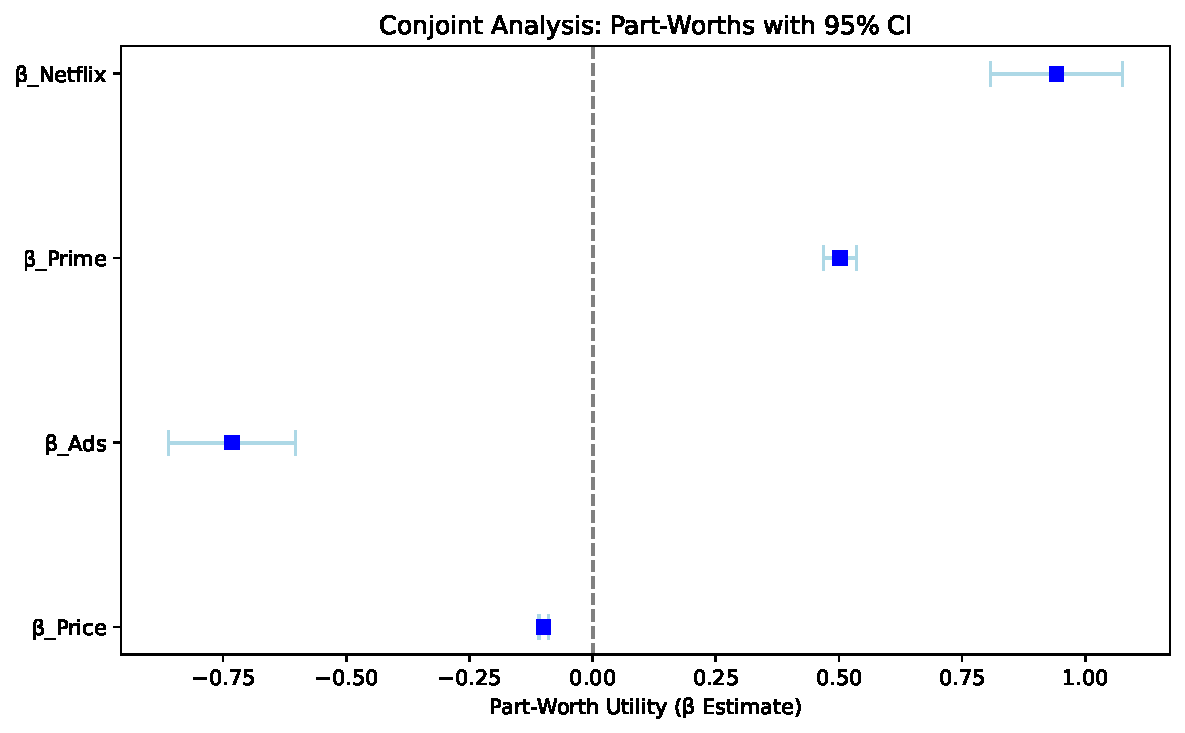
\includegraphics[keepaspectratio]{index_files/figure-pdf/cell-6-output-1.pdf}}

This analysis demonstrates that the MNL model successfully recovers
intuitive patterns of consumer preferences across different attribute
levels.

\subsection{5. Estimation via Bayesian
Methods}\label{estimation-via-bayesian-methods}

To estimate the posterior distribution of the part-worth parameters, we
implemented a Metropolis-Hastings Markov Chain Monte Carlo (MCMC)
sampler. The proposal distribution for the sampler was a multivariate
normal with zero mean and diagonal covariance, corresponding to four
independent normal proposals: three with standard deviation 0.05 (for
the binary variables: brand and ad), and one with standard deviation
0.005 (for the continuous price variable). The priors for the parameters
were set as:

\begin{itemize}
\tightlist
\item
  \(\beta_{\text{Netflix}},\ \beta_{\text{Prime}},\ \beta_{\text{Ads}} \sim \mathcal{N}(0,\ 5^2)\)
\item
  \(\beta_{\text{Price}} \sim \mathcal{N}(0,\ 1^2)\)
\end{itemize}

We ran the sampler for 11,000 iterations and discarded the first 1,000
as burn-in, retaining the remaining 10,000 samples to approximate the
posterior distribution.

\begin{Shaded}
\begin{Highlighting}[]
\KeywordTok{def}\NormalTok{ log\_prior(beta):}
    \CommentTok{\# beta: [β\_Netflix, β\_Prime, β\_Ads, β\_Price]}
\NormalTok{    logp }\OperatorTok{=} \DecValTok{0}
\NormalTok{    logp }\OperatorTok{+=} \OperatorTok{{-}}\FloatTok{0.5} \OperatorTok{*}\NormalTok{ (beta[}\DecValTok{0}\NormalTok{]}\OperatorTok{**}\DecValTok{2}\NormalTok{) }\OperatorTok{/} \DecValTok{25}  \CommentTok{\# N(0,5²)}
\NormalTok{    logp }\OperatorTok{+=} \OperatorTok{{-}}\FloatTok{0.5} \OperatorTok{*}\NormalTok{ (beta[}\DecValTok{1}\NormalTok{]}\OperatorTok{**}\DecValTok{2}\NormalTok{) }\OperatorTok{/} \DecValTok{25}
\NormalTok{    logp }\OperatorTok{+=} \OperatorTok{{-}}\FloatTok{0.5} \OperatorTok{*}\NormalTok{ (beta[}\DecValTok{2}\NormalTok{]}\OperatorTok{**}\DecValTok{2}\NormalTok{) }\OperatorTok{/} \DecValTok{25}
\NormalTok{    logp }\OperatorTok{+=} \OperatorTok{{-}}\FloatTok{0.5} \OperatorTok{*}\NormalTok{ (beta[}\DecValTok{3}\NormalTok{]}\OperatorTok{**}\DecValTok{2}\NormalTok{) }\OperatorTok{/} \DecValTok{1}   \CommentTok{\# N(0,1²)}
    \ControlFlowTok{return}\NormalTok{ logp}

\KeywordTok{def}\NormalTok{ log\_posterior(beta, X, y, group\_ids):}
    \ControlFlowTok{return}\NormalTok{ log\_likelihood(beta, X, y, group\_ids) }\OperatorTok{+}\NormalTok{ log\_prior(beta)}

\KeywordTok{def}\NormalTok{ metropolis\_sampler(X, y, group\_ids, n\_draws}\OperatorTok{=}\DecValTok{11000}\NormalTok{):}
\NormalTok{    np.random.seed(}\DecValTok{42}\NormalTok{)}
\NormalTok{    beta\_current }\OperatorTok{=}\NormalTok{ np.zeros(}\DecValTok{4}\NormalTok{)}
\NormalTok{    samples }\OperatorTok{=}\NormalTok{ []}
\NormalTok{    acc }\OperatorTok{=} \DecValTok{0}

    \ControlFlowTok{for}\NormalTok{ i }\KeywordTok{in} \BuiltInTok{range}\NormalTok{(n\_draws):}
        \CommentTok{\# proposal: 4 independent normals}
\NormalTok{        proposal }\OperatorTok{=}\NormalTok{ beta\_current }\OperatorTok{+}\NormalTok{ np.random.normal(loc}\OperatorTok{=}\DecValTok{0}\NormalTok{, scale}\OperatorTok{=}\NormalTok{[}\FloatTok{0.05}\NormalTok{, }\FloatTok{0.05}\NormalTok{, }\FloatTok{0.05}\NormalTok{, }\FloatTok{0.005}\NormalTok{])}

        \CommentTok{\# compute log{-}posterior}
\NormalTok{        log\_post\_curr }\OperatorTok{=}\NormalTok{ log\_posterior(beta\_current, X, y, group\_ids)}
\NormalTok{        log\_post\_prop }\OperatorTok{=}\NormalTok{ log\_posterior(proposal, X, y, group\_ids)}

        \CommentTok{\# acceptance probability}
\NormalTok{        log\_alpha }\OperatorTok{=}\NormalTok{ log\_post\_prop }\OperatorTok{{-}}\NormalTok{ log\_post\_curr}
        \ControlFlowTok{if}\NormalTok{ np.log(np.random.rand()) }\OperatorTok{\textless{}}\NormalTok{ log\_alpha:}
\NormalTok{            beta\_current }\OperatorTok{=}\NormalTok{ proposal}
\NormalTok{            acc }\OperatorTok{+=} \DecValTok{1}
\NormalTok{        samples.append(beta\_current.copy())}

    \BuiltInTok{print}\NormalTok{(}\SpecialStringTok{f"Acceptance rate: }\SpecialCharTok{\{}\NormalTok{acc}\OperatorTok{/}\NormalTok{n\_draws}\SpecialCharTok{:.3f\}}\SpecialStringTok{"}\NormalTok{)}
    \ControlFlowTok{return}\NormalTok{ np.array(samples[}\DecValTok{1000}\NormalTok{:])  }\CommentTok{\# burn{-}in: discard first 1000}
\end{Highlighting}
\end{Shaded}

The acceptance rate of the sampler was approximately 56.7\%, which
indicates good mixing without excessive rejection. Summary statistics of
the posterior draws are shown below:

\begin{Shaded}
\begin{Highlighting}[]
\NormalTok{samples }\OperatorTok{=}\NormalTok{ metropolis\_sampler(x, y, group\_ids)}

\NormalTok{param\_names }\OperatorTok{=}\NormalTok{ [}\StringTok{\textquotesingle{}β\_Netflix\textquotesingle{}}\NormalTok{, }\StringTok{\textquotesingle{}β\_Prime\textquotesingle{}}\NormalTok{, }\StringTok{\textquotesingle{}β\_Ads\textquotesingle{}}\NormalTok{, }\StringTok{\textquotesingle{}β\_Price\textquotesingle{}}\NormalTok{]}
\ControlFlowTok{for}\NormalTok{ i }\KeywordTok{in} \BuiltInTok{range}\NormalTok{(}\DecValTok{4}\NormalTok{):}
\NormalTok{    mean }\OperatorTok{=}\NormalTok{ samples[:, i].mean()}
\NormalTok{    sd }\OperatorTok{=}\NormalTok{ samples[:, i].std()}
\NormalTok{    ci }\OperatorTok{=}\NormalTok{ np.percentile(samples[:, i], [}\FloatTok{2.5}\NormalTok{, }\FloatTok{97.5}\NormalTok{])}
    \BuiltInTok{print}\NormalTok{(}\SpecialStringTok{f"}\SpecialCharTok{\{}\NormalTok{param\_names[i]}\SpecialCharTok{\}}\SpecialStringTok{: mean=}\SpecialCharTok{\{}\NormalTok{mean}\SpecialCharTok{:.3f\}}\SpecialStringTok{, sd=}\SpecialCharTok{\{}\NormalTok{sd}\SpecialCharTok{:.3f\}}\SpecialStringTok{, 95\% CI=}\SpecialCharTok{\{}\NormalTok{ci}\SpecialCharTok{\}}\SpecialStringTok{"}\NormalTok{)}
\end{Highlighting}
\end{Shaded}

\begin{verbatim}
Acceptance rate: 0.567
β_Netflix: mean=0.946, sd=0.113, 95% CI=[0.73207093 1.17071416]
β_Prime: mean=0.507, sd=0.114, 95% CI=[0.28823335 0.7350442 ]
β_Ads: mean=-0.733, sd=0.083, 95% CI=[-0.89090517 -0.56675583]
β_Price: mean=-0.100, sd=0.006, 95% CI=[-0.11186317 -0.0873375 ]
\end{verbatim}

The posterior means are nearly identical to the MLE estimates obtained
earlier, and the posterior standard deviations align closely with the
standard errors from the MLE. This consistency confirms the convergence
and validity of the Bayesian approach.

Below, we present a trace plot and posterior histogram for β\_Netflix,
which demonstrate both good convergence and approximately normal
posterior shape:

\begin{Shaded}
\begin{Highlighting}[]
\NormalTok{plt.figure(figsize}\OperatorTok{=}\NormalTok{(}\DecValTok{12}\NormalTok{, }\DecValTok{5}\NormalTok{))}

\CommentTok{\# trace}
\NormalTok{plt.subplot(}\DecValTok{1}\NormalTok{, }\DecValTok{2}\NormalTok{, }\DecValTok{1}\NormalTok{)}
\NormalTok{plt.plot(samples[:, }\DecValTok{0}\NormalTok{])}
\NormalTok{plt.title(}\StringTok{"Trace plot: β\_Netflix"}\NormalTok{)}

\CommentTok{\# posterior histogram}
\NormalTok{plt.subplot(}\DecValTok{1}\NormalTok{, }\DecValTok{2}\NormalTok{, }\DecValTok{2}\NormalTok{)}
\NormalTok{plt.hist(samples[:, }\DecValTok{0}\NormalTok{], bins}\OperatorTok{=}\DecValTok{30}\NormalTok{, density}\OperatorTok{=}\VariableTok{True}\NormalTok{, color}\OperatorTok{=}\StringTok{\textquotesingle{}skyblue\textquotesingle{}}\NormalTok{)}
\NormalTok{plt.title(}\StringTok{"Posterior of β\_Netflix"}\NormalTok{)}
\NormalTok{plt.show()}
\end{Highlighting}
\end{Shaded}

\pandocbounded{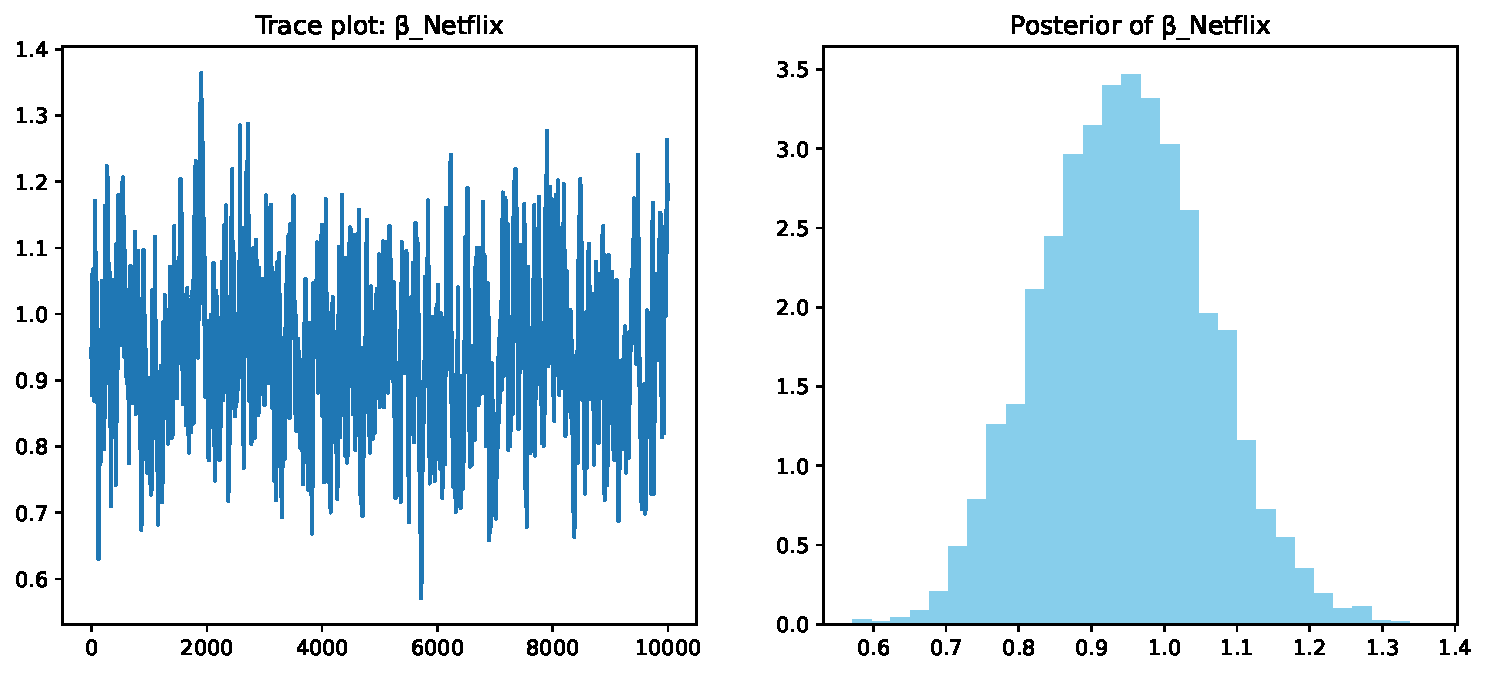
\includegraphics[keepaspectratio]{index_files/figure-pdf/cell-10-output-1.pdf}}

These diagnostics suggest that the MCMC sampler is well-calibrated and
effectively captures the uncertainty in the parameter estimates. The
posterior distributions provide a full probabilistic characterization of
the model parameters, offering richer information than point estimates
alone.

Overall, the Bayesian estimates reaffirm the conclusions drawn from the
MLE approach, while offering additional insight into the uncertainty and
shape of the posterior distributions.

\subsection{6. Discussion}\label{discussion}

\subsubsection{Interpreting Estimated
Preferences}\label{interpreting-estimated-preferences}

When interpreting the estimated coefficients from the multinomial logit
model, we observe that the utility weight for Netflix is substantially
higher than that for Prime, indicating that, all else equal, respondents
have a stronger preference for Netflix over Prime. This ranking is
consistent with expectations in a realistic streaming market where
Netflix is often perceived as offering superior content or usability.

The coefficient on Ads is negative, suggesting that respondents derive
lower utility from ad-supported offerings compared to ad-free
experiences. This aligns well with known consumer aversion to
advertising interruptions in digital media consumption.

In addition, the coefficient for Price is negative, which is both
statistically significant and economically intuitive: higher prices
reduce utility, making the option less attractive. The monotonic
relationship between price and utility is a foundational assumption in
discrete choice models, and our estimates support this behavior.

Taken together, these results offer a coherent picture of consumer
preferences: respondents tend to favor Netflix over Prime and Hulu (the
omitted baseline), prefer content without ads, and exhibit price
sensitivity. Importantly, these preferences emerge solely from the
observed choice data, without requiring knowledge of how the data was
originally simulated.

\subsubsection{Extending to a Hierarchical
Model}\label{extending-to-a-hierarchical-model}

To move from a standard multinomial logit model to a multi-level
(hierarchical or random-coefficients) model, one would need to allow for
heterogeneity in preferences across individuals. Rather than assuming a
single set of fixed coefficients shared by all respondents, a
hierarchical model assumes that each respondent has their own set of
utility weights, denoted by βᵢ. These individual-level coefficients are
not estimated independently, but are instead assumed to be drawn from a
common population-level distribution:

\[
\beta_i \sim \mathcal{N}(\mu, \Sigma)
\]

Here, μ represents the average part-worth utilities across the
population, and Σ captures the variability (and possible covariation) in
preferences between respondents. This structure enables the model to
account for observed choice variation that arises from true preference
differences, rather than attributing all variation to random error.

To simulate such data, one would first sample respondent-specific βᵢ
vectors from the population distribution, and then use those to generate
choices under the standard multinomial logit framework. Estimation of
this hierarchical model typically involves Bayesian methods, such as
hierarchical Bayes using Gibbs sampling or Hamiltonian Monte Carlo,
which jointly infer both the individual-level parameters and the
hyperparameters (μ, Σ).

This modeling approach is widely used in real-world conjoint analysis
because it captures individual-level heterogeneity, provides more
accurate preference predictions, and allows richer segmentation and
targeting insights than fixed-effects models.




\end{document}
